\chapter{Testing and Characterization}
    \section{Detecting}
        A detailed description of each individual parameter can be found in the~\cite{Manual.HandelAPIManual.Xiang,Manual.HandelProgrammersGuideMicroDXP.Xiang,Software.HandelRelease.2023}.

        \begin{lstlisting}[style=mypython,
            caption={[]Detector settings taken from the technical specifications report coming with the detector. If not stated otherwise the value stored on the device was used.},
            label={lst:default detection parameters}]
    params = {
        "parset":     2.400000, # 2.000000
        # "genset":     0.000000,
        # "fippi":     0.000000,
        "clock_speed":    40.000000,
        "energy_gap_time":     0.300000, # 0.3
        "trigger_peak_time":     0.050000,
        "trigger_gap_time":     0.000000,
        "baseline_length":     512.000000, # 512.000000
        "trigger_threshold":   150.000000, # 100.000000
        "baseline_threshold":   120.000000, # 120.000000
        "energy_threshold":     0.000000, # 0.000000
        "peak_interval_offset":     0.500000,
        "peak_sample_offset":     0.000000,
        "max_width":     0.400000,
        "peak_mode":     0.000000,
        "peak_interval":     0.500000,
        "peak_sample":     0.000000,
        "polarity":     1.000000,
        "preamp_value":     1.000000, # reset interval in us
        "gain":     4.484848, # 3.639965
        "gain_trim":     1.000000, # 1.018982
        "number_mca_channels":  8192.000000,
        "mca_bin_width":     1.000000,
        "bytes_per_bin":     3.000000,
        "adc_trace_wait":     0.025000,
        "auto_adjust_offset":     1.000000,
        "number_of_scas":     0.000000,
    }
        \end{lstlisting}

        \texttt{gain} is set to \qty{4.484848}{\volt} according to

        \begin{align}
            gain = \frac{1184}{DynRange \cdot PreampValue}
        \end{align}

        with \(DynRange = \qty{40}{\kV}\) and \(PreampValue = \qty{6.6}{\volt\per\kV}\).

        \begin{figure}[h]
            \centering
            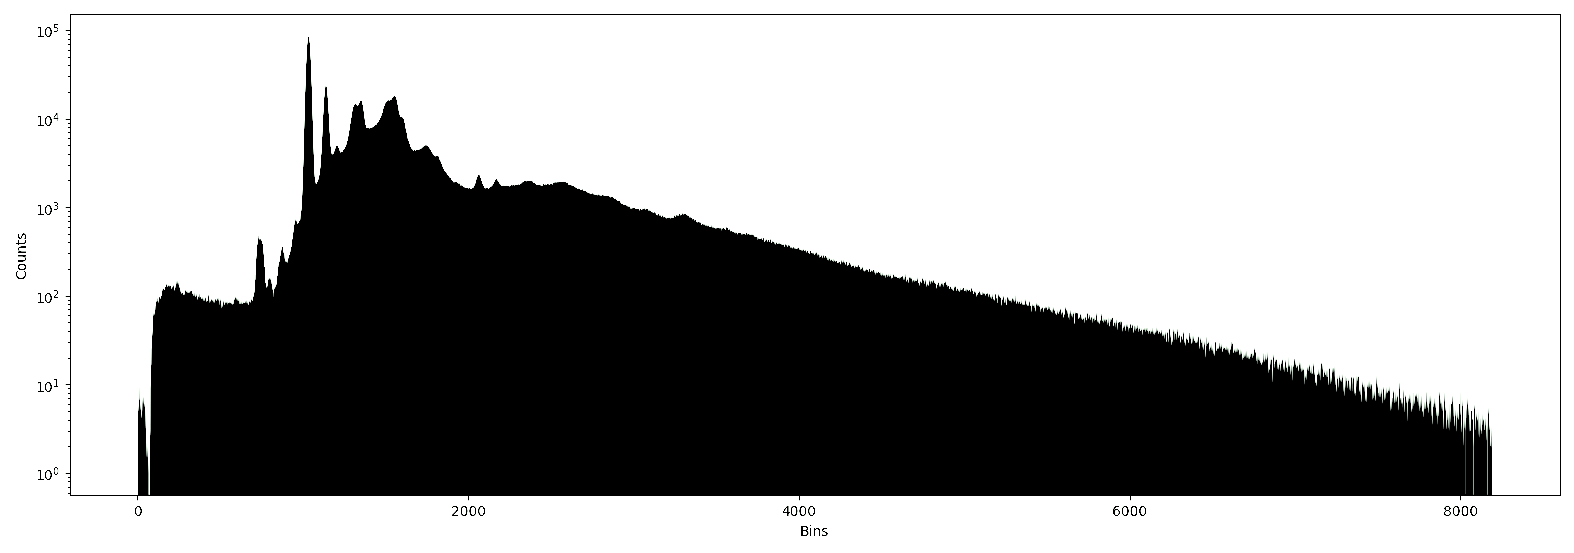
\includegraphics[width=\textwidth]{spectra/steel40kV.png}
            \caption[short]{Spectrum taken against a chunk of steel at \qty{40}{\kV} using the settings specified in \cref{lst:default detection parameters}.}%
            \label{fig:spectrum steel 40kV}
        \end{figure}

        The spectrum shown in \cref{fig:spectrum steel 40kV} is not yet calibrated.
        Yet, with reasonable confidence it is assumed the peaks visible between bins 1000 and 2000 originate from Fe-\(K\alpha_1\) and Fe-\(K\alpha_2\) as well some Cu and Zn lines from the tubes outer material.
        Lastly the hump at the far left and the barely visible peaks right after bin 2000 presumably originate from the tungsten target.

    \section{Angular Resolution}
        The angular resolution for each individual stage is given by \cref{eq:angular resolution}

        \begin{align}
            res_{\angle} &= \frac{360}{microsteps \cdot fullStepsPerRevolution} \cdot gearRatio
            \label{eq:angular resolution}
        \end{align}

        and yields

        \begin{align}
            res_{\varphi} = \frac{\qty{360}{\degree}}{32 \cdot \qty{200}{\step}} \cdot \frac{80}{250} = \qty{0.018}{\degree\per\step}
        \end{align}

        for the detector stage and

        \begin{align}
            res_{\Theta} = \frac{\qty{360}{\degree}}{32 \cdot \cdot \qty{200}{\step}} \cdot \frac{20}{80} \approx \qty{0.0141}{\degree\per\step}
        \end{align}